\documentclass[a4paper,12pt,abstracton,titlepage]{scrartcl}

\usepackage[french]{babel}
%\usepackage[T1]{fontenc}
\usepackage[utf8]{inputenc} % Umlaute, evtl. vom Betriebssystem abhaengig
\usepackage{lmodern}
\usepackage{pgfgantt}
\usepackage{titlesec}
\usepackage{float}
\usepackage{floatflt}
\usepackage{blindtext}
\usepackage{amsmath}
\usepackage{tabularx,url}
\usepackage[a4paper, left=2cm, textwidth=17cm, top=1.5cm]{geometry}
\usepackage{hyperref}
\usepackage{longtable}


\titleformat*{\section}{\large\bfseries}
\titleformat*{\subsection}{\large\bfseries}
\titleformat*{\subsubsection}{\large\bfseries}
\titleformat*{\paragraph}{\large\bfseries}
\titleformat*{\subparagraph}{\large\bfseries}

\renewcaptionname{french}{\figurename}{Fig.}

%\titlehead{Ulm University}
%\title{Title}
%\subject{Subject}
%\author{Author}
%\publishers{%
	%\rule{\textwidth}{0.4pt} \\
	%\vspace{0.5cm}
    %\normalfont\normalsize%
    %\parbox{0.9\linewidth}{%
    %    Abstract or Introduction
    %} \\
    %\vspace{0.5cm}
   	%\rule{\textwidth}{0.4pt}
%}
\title{Partajeux}
\date{26 janvier 2018}
%\author{DANG Hung Hoang,\\FUDITPHU Yan-Guillaume,\\KULZER Ulrike}
\author{John Doe\\ Magic Department, Richard Miles University
        \and Richard Row, \LaTeX\ Academy}

\renewcommand*\contentsname{Summary}

\begin{document}
%\maketitle

\begin{titlepage}
	\centering
	{\LARGE ESIEE Paris\par}
	\vspace{1cm}
	{\scshape\Large SI-4301B Architecture et développement d’applications Web en PHP\par}
	\vfill
	{\huge\bfseries Partajeux\par}
	\vfill
	{\large DANG Hung Hoang, FUDITPHU Yan-Guillaume, KULZER Ulrike\par}

\end{titlepage}



%%% begin costom title
{\Large\noindent \emph{ESIEE Paris}}

{\Large\noindent \emph{SI-4301B}}
\vspace{1cm}
\begin{center}
	{\huge \textbf{Partajeux}
	\\
	\vspace{0.3cm}
	\large DANG Hung Hoang, FUDITPHU Yan-Guillaume, KULZER Ulrike
	\\
	\vspace{0.2cm}
	\today}
\end{center}
%%% end custom title
\vspace{1cm}
%\maketitle
\tableofcontents

\setcounter{page}{1} % reset page counter to one for the first page, leave the title page out

\newpage
\section{Présentation du projet}
\subsection{Introduction/Description}
\vspace{0.2cm}
{\Large Partajeux\\}

Est une plateforme de mise en relation qui permet aux utilisateurs d'échanger
pour une durée de temps leur jeux vidéo en ligne. Ils déterminent grâce à
l'application les jeux qu'ils veulent échanger, puis fixent un rendez vous (date, heure, lieu de l'échange, durée).//
L'utilisateur doit pouvoir se connecter à l'application, s'identifier, ajouter ses jeux à échanger et ajouter des jeux voulu. L'utilisateur pourra rechercher les jeux qu'il veut et l'application affichera les utilisateurs qui peuvent potentiellement échanger (ils sont soit intéressés par un de nos jeux, soit ils ont la console pour un de nos jeux). L'utilisateur pourra ensuite proposer un échange et attendra la confirmation. Lorsque l'échange s'effectue les utilisateurs confirment l'échange et les jeux deviennent indisponible. Lorsque la durée de l'échange est terminé les utilisateurs doivent confirmer le retour des jeux pour qu'ils redeviennent disponible dans l'application.\\

Sites d'inspiration:\\
\begin{itemize}
\item Steam : 
\url{http://store.steampowered.com/}\\
\item Romstation : 
\url{http://www.romstation.fr/accueil}\\
\item Smiile : 
\url{https://www.smiile.com/}\\
\item MyTroc : 
\url{https://mytroc.fr/}\\
\item GchangeTout : 
\url{http://www.gchangetout.com/}\\
\item Ebay : 
\url{https://www.ebay.fr/}\\
\item LeBonCoin : 
\url{https://www.leboncoin.fr/}\\
\end{itemize}

\subsection{L'équipe}
% experiences
L'équipe de Partajeux se compose de trois membres :\\
\begin{itemize}
\item Hung Hoang DANG : expérimenté en développement web et SQL\\
\item Yan-Guillaume FUDITPHU : expérimenté en développement web et SQL\\
\item Ulrike KULZER : expérimentée en SQL\\
\end{itemize}



\newpage
\section{Analyse fonctionnelle}
\begin{longtable}{|p{0.23\textwidth}|p{0.25\textwidth}|p{0.25\textwidth}|l|}
\hline
\textbf{Fonctionnalité} & \textbf{Tâche} & \textbf{Sous-tâche} & \textbf{Importance}\\
\hline
Page de connexion & Formulaire d'inscription & Nom d'utilisateur & *****\\
 \hline
 & & Adresse Mail & *****\\
 \hline
 & & Mot de passe & *****\\
 \hline
 & & Taper deux fois & **\\
 \hline
 & & & \\
 \hline
 & Formulaire de connexion & Nom d'utilisateur & *****\\
 \hline
 & & Mot de passe & *****\\
 \hline
 & & Adress mail idenfiant & * \\
 \hline
  & & & \\
 \hline	
 & Description de l'application & Texte & ****\\
 \hline
 & & Image & **\\
 \hline
  & & & \\
 \hline
  & Information (Mention légale) &  Texte & ***\\
 \hline
 & & & \\
 \hline
 & & & \\
 \hline
Page d'accueil & Vous êtes connecté en tant que & & *****\\
 \hline
& Mes jeux & & *****\\
 \hline
& Jeux voulu & & *****\\
 \hline
& Barre de recherche & & *****\\
 \hline
& Notification & & ***\\
 \hline
  & & & \\
 \hline
 & & & \\
 \hline
Page de profil & Changer mot de passe & & *****\\
 \hline
 & Changer adresse mail & & *****\\
 \hline
 & Changer/ajouter photo de profil & & *\\
 \hline
 & bloquer utilisateur & & *\\
 \hline
 & & & \\
 \hline
 & & & \\
 \hline
Page de recherche & afficher résultat & afficher le jeu (titre, console, année,...) & *****\\
\hline
 &  & afficher les users dont l'échange est possible & *****\\
 \hline
 & afficher les propositions de résultats en temps réel &  & **\\
 \hline
 & & & \\
 \hline
 & & & \\
 \hline
Page description jeu & Image &  & ****\\
 \hline
 & Titre &  & *****\\
 \hline
 & Console &  & *****\\
 \hline
 & Année &  & ***\\
 \hline
 & Description &  & ******\\
 \hline
 & Proposition d'échange &  & ******\\
 \hline
 & & & \\
 \hline
 & & & \\
 \hline
Formulaire d'échange & Lieu &  & *****\\
\hline
 & Date et heure &  & *****\\
 \hline
 & Durée de l'échange &  & *****\\
 \hline
 & Jeux échangés &  & *****\\
 \hline
 & Noms des utilisateurs &  & *****\\
 \hline
 & Bouton confirmation et envoi à l'autre utilisateur &  & *****\\
 \hline
 & Pouvoir modifier la proposition (exemple : heure) et la renvoyer &  & ****\\
 \hline
 & Champ de texte &  & *****\\
  \hline
\end{longtable}


\section{Modèle conceptuel de données}
\vspace{0.5cm}
% E-R-Diagramme
\begin{minipage}[c]{\textwidth}
\centering
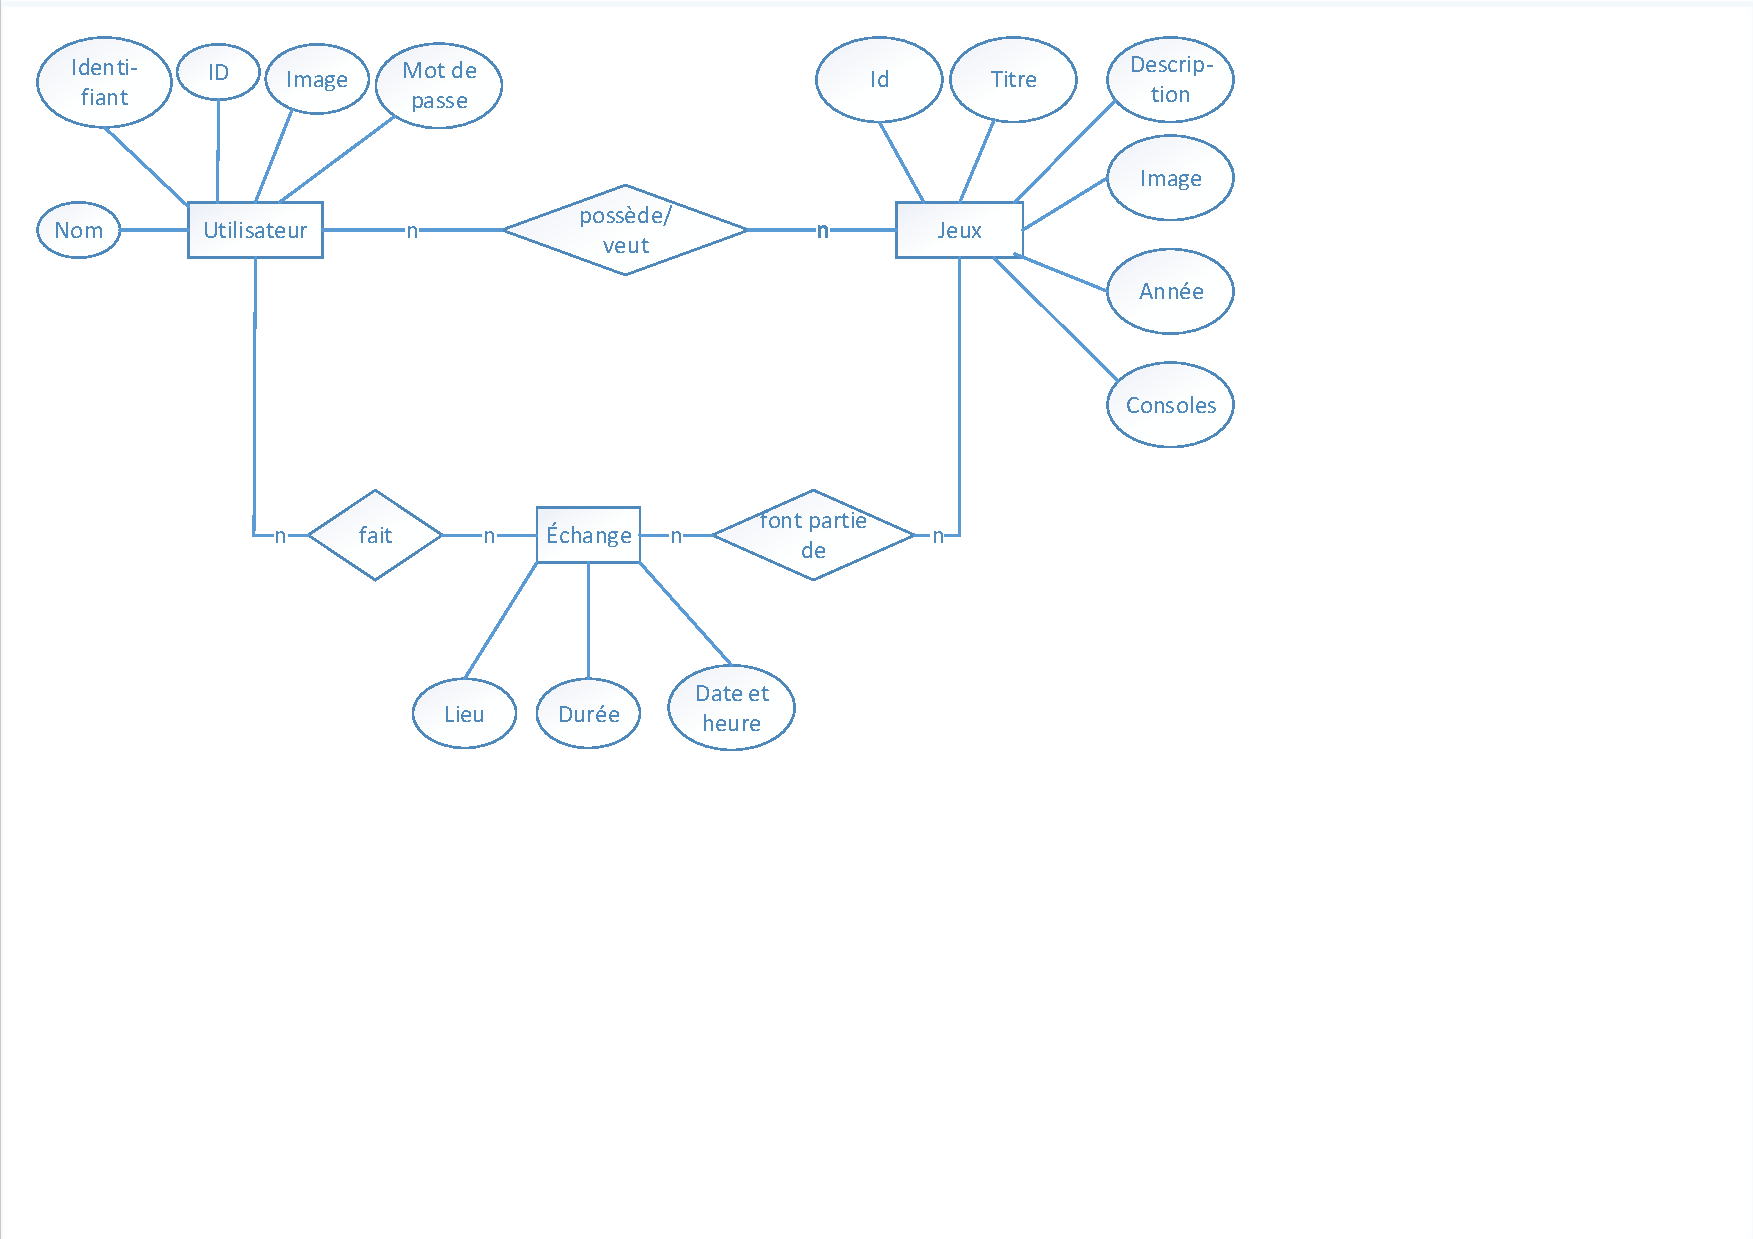
\includegraphics[width=\textwidth, trim=5mm 80mm 80mm 5mm, clip]{./doc/E-R-Diagrammme.pdf}
    %TRIM = LINKS UNTEN RECHTS OBEN
\captionof{figure}{Modèle entité-association au début du projet}
\label{img:er}
\vspace{1cm}

% Modèle conceptuel de données FINALE
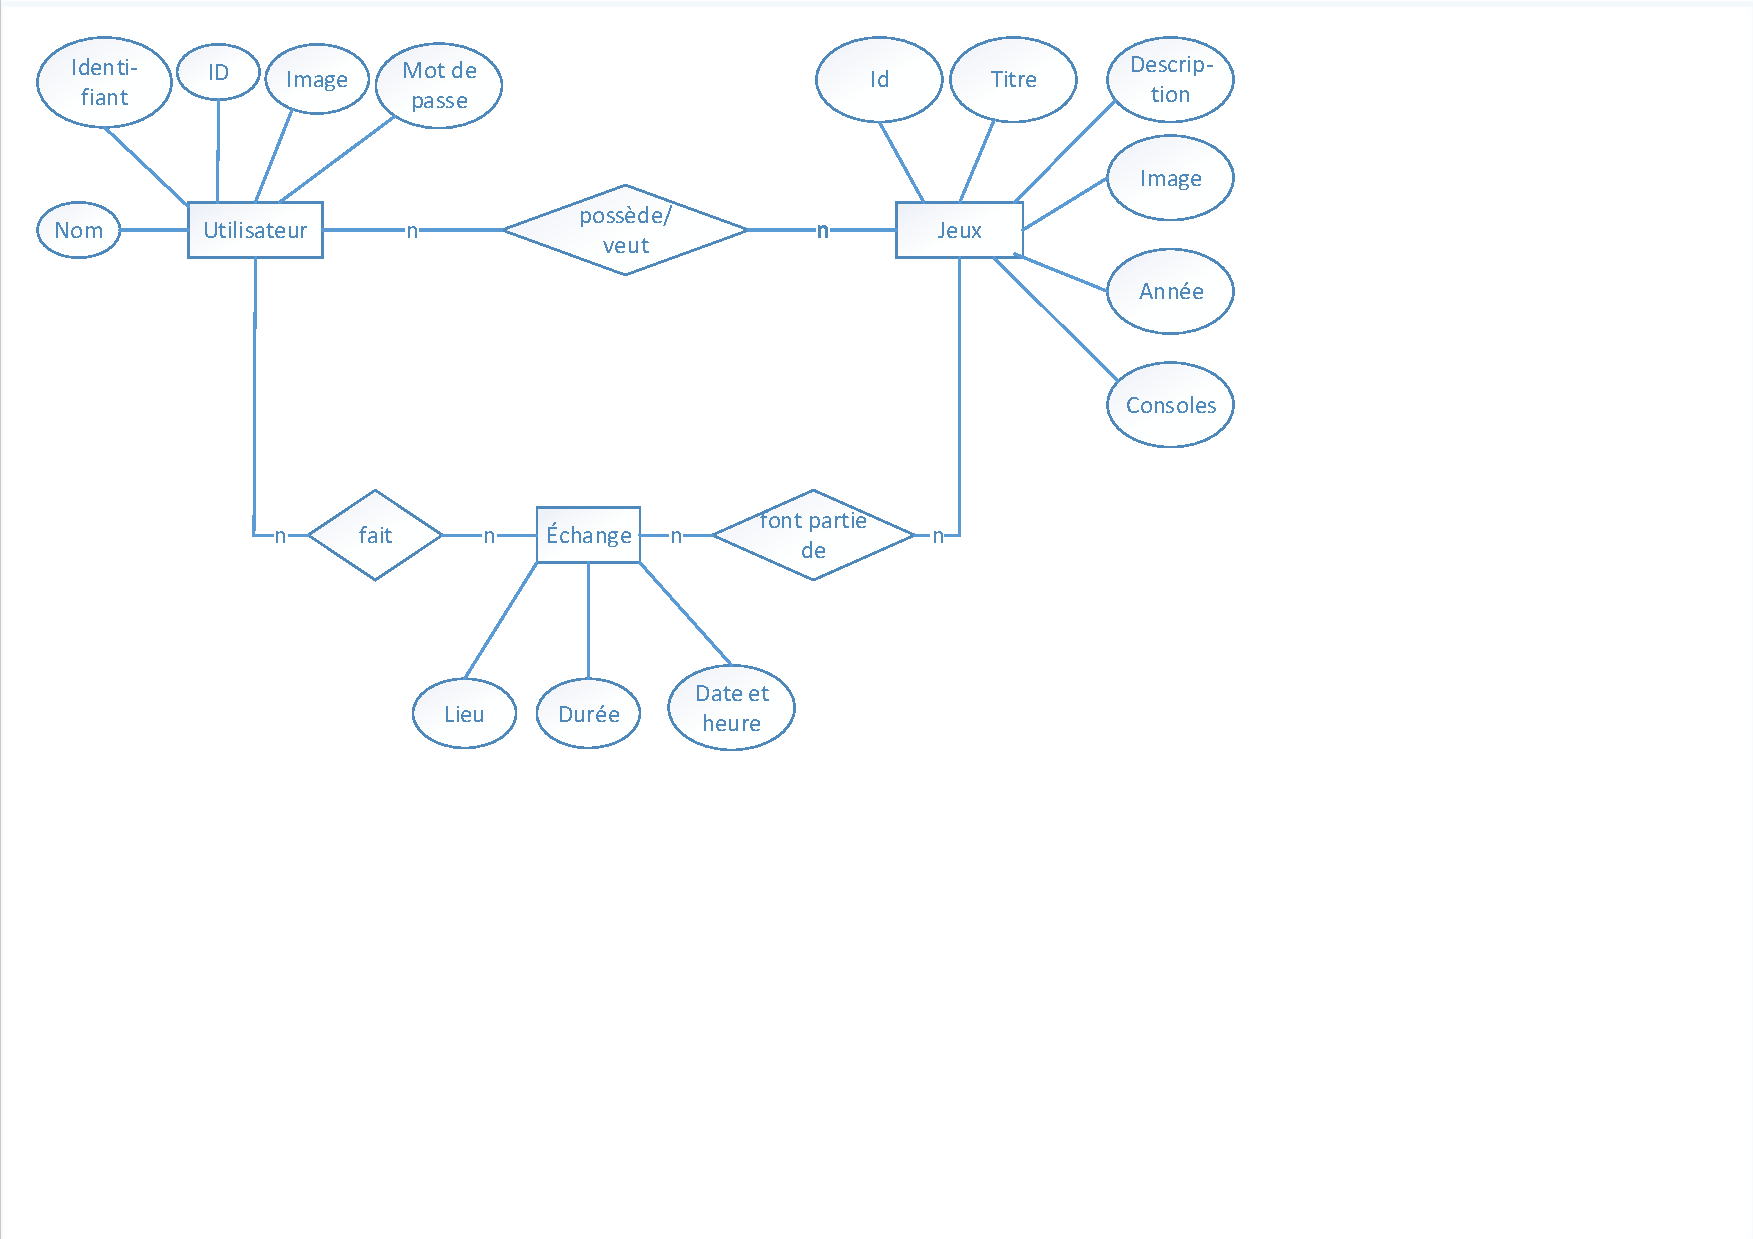
\includegraphics[width=\textwidth, trim=5mm 80mm 80mm 5mm, clip]{./doc/E-R-Diagrammme.pdf}
    %TRIM = LINKS UNTEN RECHTS OBEN
\captionof{figure}{Modèle conceptuel de données à la fin du projet}
\label{img:mcd}
\end{minipage}

\newpage
\section{Documentation}
\subsection{Documentation technique}
\subsubsection{Organisation}
\begin{floatingfigure}[r]{0.25\textwidth}

\includegraphics[width=0.15\textwidth]{./doc/git_logo.png}
%\caption{Le logo de git}
\label{git}
\end{floatingfigure}

Pour mieux nous organiser et échanger le code du programme nous avons décidé d'utiliser git. Git est un système de contrôle de versions distribuées gratuit qui était créé pour gérer vite et efficacement les projets de toutes les tailles. Pour notre projet nous avons utilisé un repository public.
Vous trouveriez plus des informations sous \url{https://github.com/} et \url{https://git-scm.com/}.\\

\subsubsection{Pré-requis et instruction d'installation}
Les pré-requis sont:  serveur Apache, Mysql 5, PHP 7.0\\
-- apache, javascript, php, html, css, mySQL, jQuery

\subsubsection{Choix d'architecture et d'implémentation particuliers}
Le site est codé avec une architecture Model-View-Controller (MVC) qui nous permet de séparer vue, modèle et les commandes de l'utilisateur.\\
Les contrôleurs reçoivent les requêtes de l'utilisateur et utilisent les fonctions du modèle afin de récupérer les informations de la base de données, le contrôleur affiche ensuite la vue avec les différentes informations. Dans ce projet les vues utilisent aussi le modèle pour accéder à la base de donnée.\\
\begin{figure}[h]
  \centering
    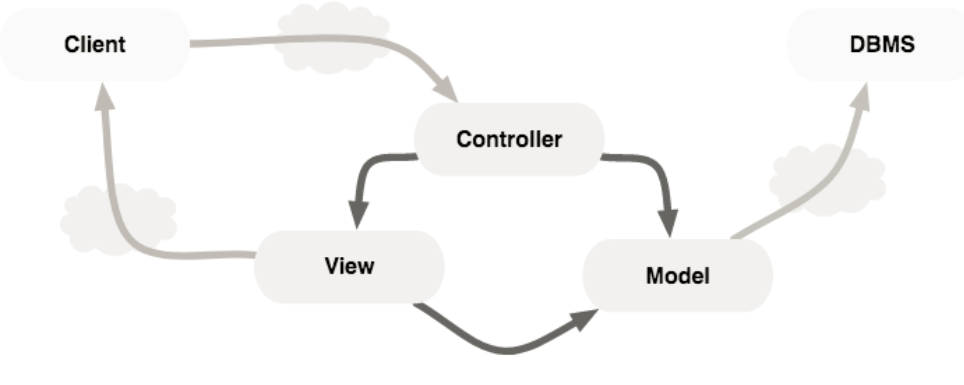
\includegraphics[width=\textwidth]{./doc/mvc.png}
	\caption{Le modèle MVC}
	\label{mvc}
\end{figure}

De plus nous avons utilisé la technologie AJAX pour la barre de recherche.\\
Nous avons décidé de ne pas utiliser de framework car nos connaissances/compétences étaient insuffisants en considérant le temps qu'il restait pour le projet.\\

\newpage
\subsection{Documentation utilisateurs}
\begin{figure}[h]
  \centering
    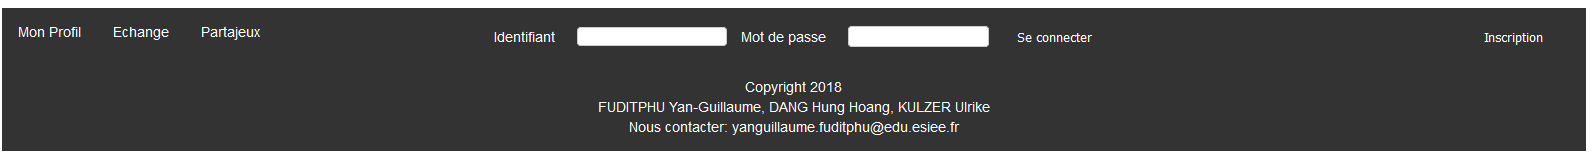
\includegraphics[width=\textwidth]{./doc/01_startscreen.png}
	\caption{Page d'accueil}
	\label{pdacc}
\end{figure}

Lorsque l'utilisateur ouvre la page de Partajeux il se retrouve sur la page d'accueil suivante (voir figure \ref{pdacc}). Ici il peut trouver plus d'informations sur Partajeux en cliquant sur le bouton "Partajeux" dans la barre de navigation ou se connecter directement avec son identifiant et mot de passe. S'il n'est pas encore inscrit il suffit de cliquer sur "Inscription" pour afficher le formulaire d'inscription:\\
\begin{figure}[h]
  \centering
    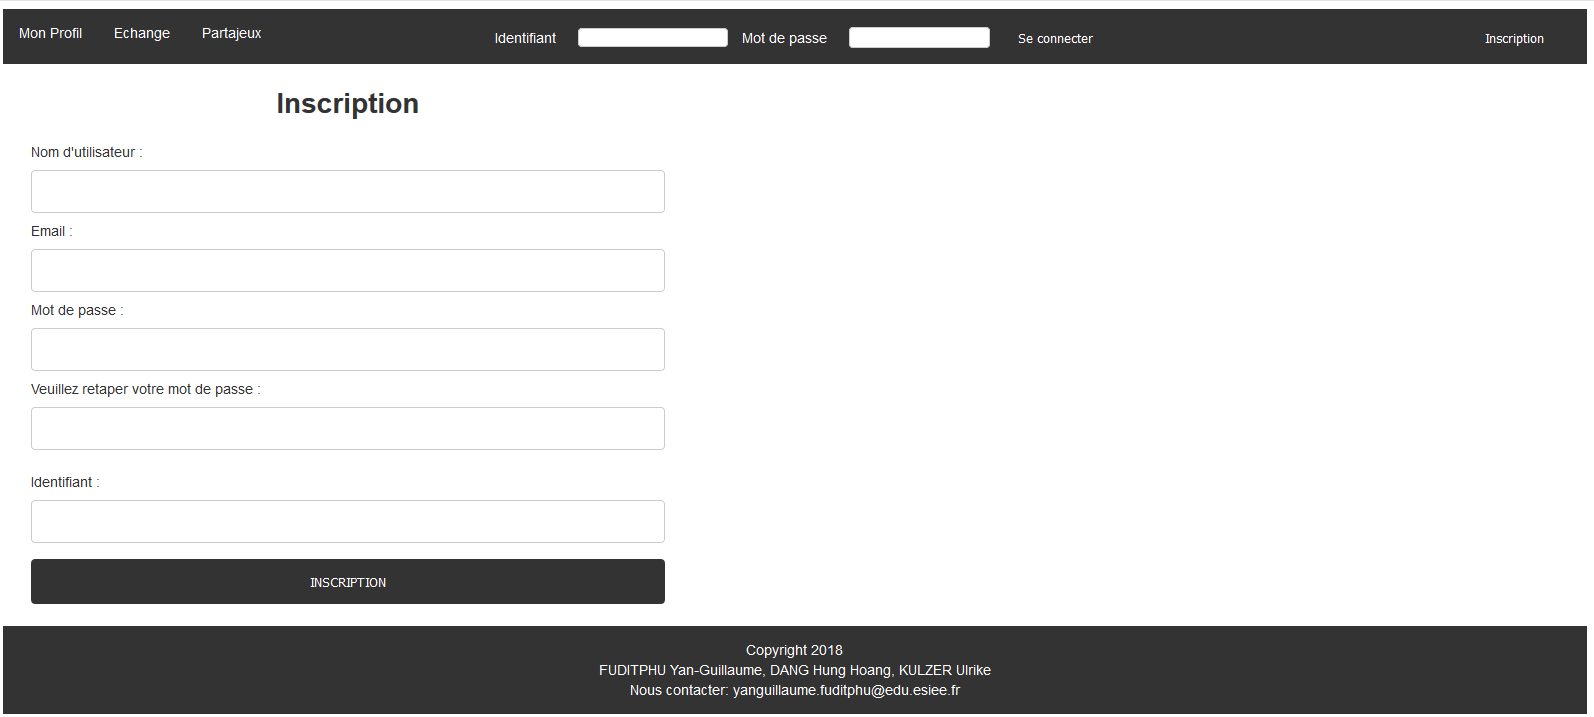
\includegraphics[width=\textwidth]{./doc/02_inscription.png}
	\caption{Formulaire d'inscription}
	\label{insc}
\end{figure}

Pour s'inscrire l'utilisateur doit mettre son nom et son adresse mail. Ensuite il choisit un identifiant qui est utilisé pour se connecter et un mot de passe qu'il doit entrer deux fois pour éviter qu'il fait une faute et qu'il ne peut plus se connecter après. Le système va chercher dans la base de données si l'identifiant est déjà pris et dans ce cas prévenir l'utilisateur.\\
Une fois inscrit et connecté, l'utilisateur peut choisir dans la barre de navigation ce qu'il veut faire:\\
\begin{itemize}
\item rechercher des jeux avec la barre de recherche qui propose des jeux correspondants à sa saisie,
\item gérer les jeux qu'il possède et ses jeux voulus en cliquant sur "Mon profil" (voir figure \ref{profile}),
\item gérer ses échanges (voir figure \ref{exch}) ou
\item se déconnecter.\\
\end{itemize}

\begin{figure}[h]
  \centering
    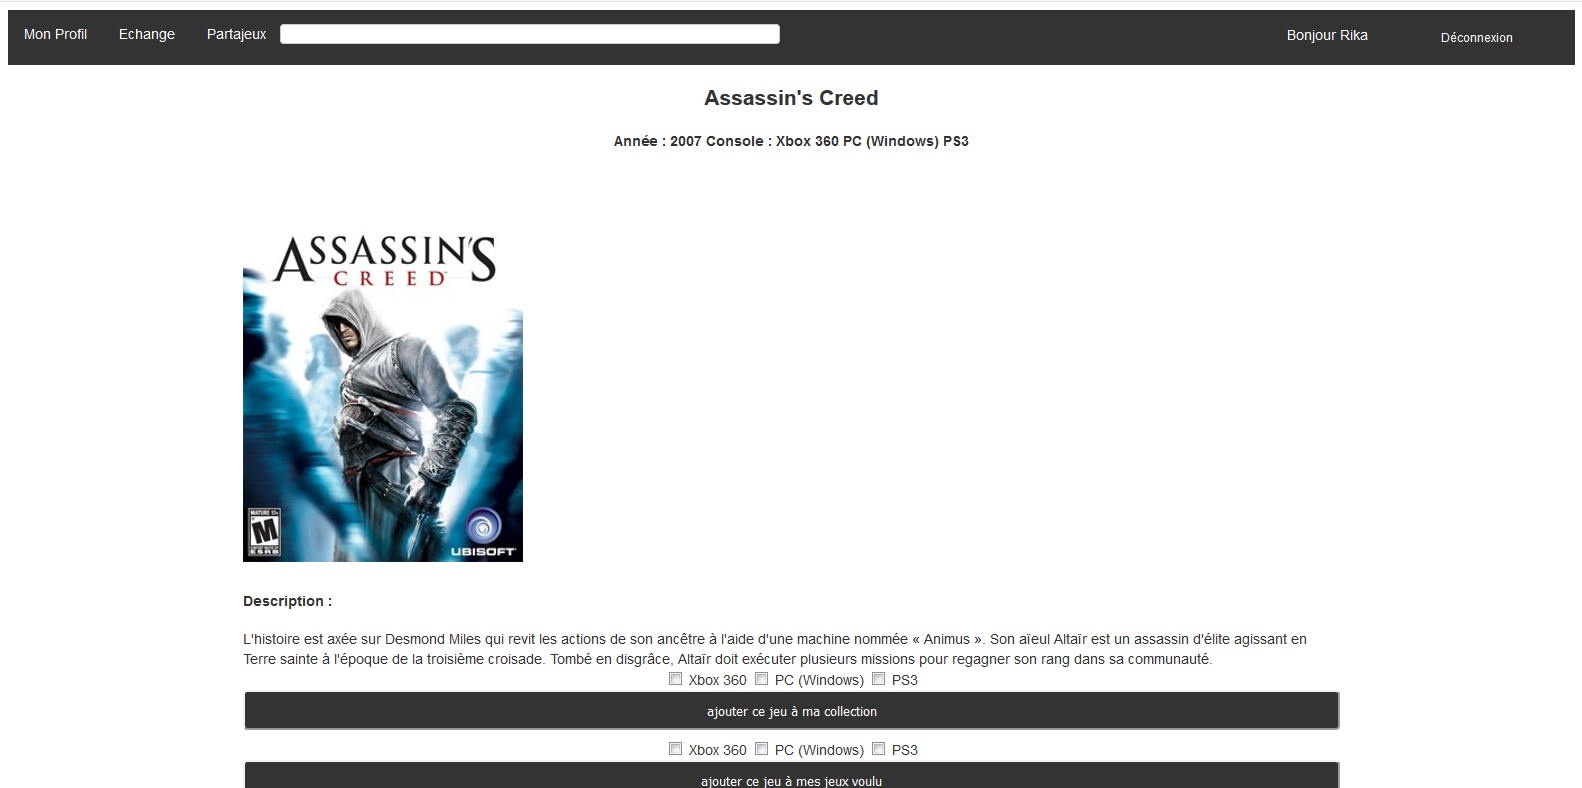
\includegraphics[width=\textwidth]{./doc/05_description_jeu.png}
	\caption{Description d'un jeu}
	\label{jeu}
\end{figure}

\newpage
Lorsque l'utilisateur clique sur un jeu proposé dans la barre de recherche la description du jeu va être affichée. Sur cette page il trouveras toutes les informations importantes sur le jeu: le titre, l'année de la sortie, les consoles pour lesquelles le jeu est sorti, une image et une brève description de l'histoire. En bas il est possible d'ajouter le jeu aux jeux possédés ou de l'ajouter aux jeux voulus. Pour réaliser une des deux actions l'utilisateur doit choisir une ou plusieurs consoles du jeux et cliquer sur le bouton correspondant à la liste souhaitée.
\vspace{1cm}
\begin{figure}[!h]
  \centering
    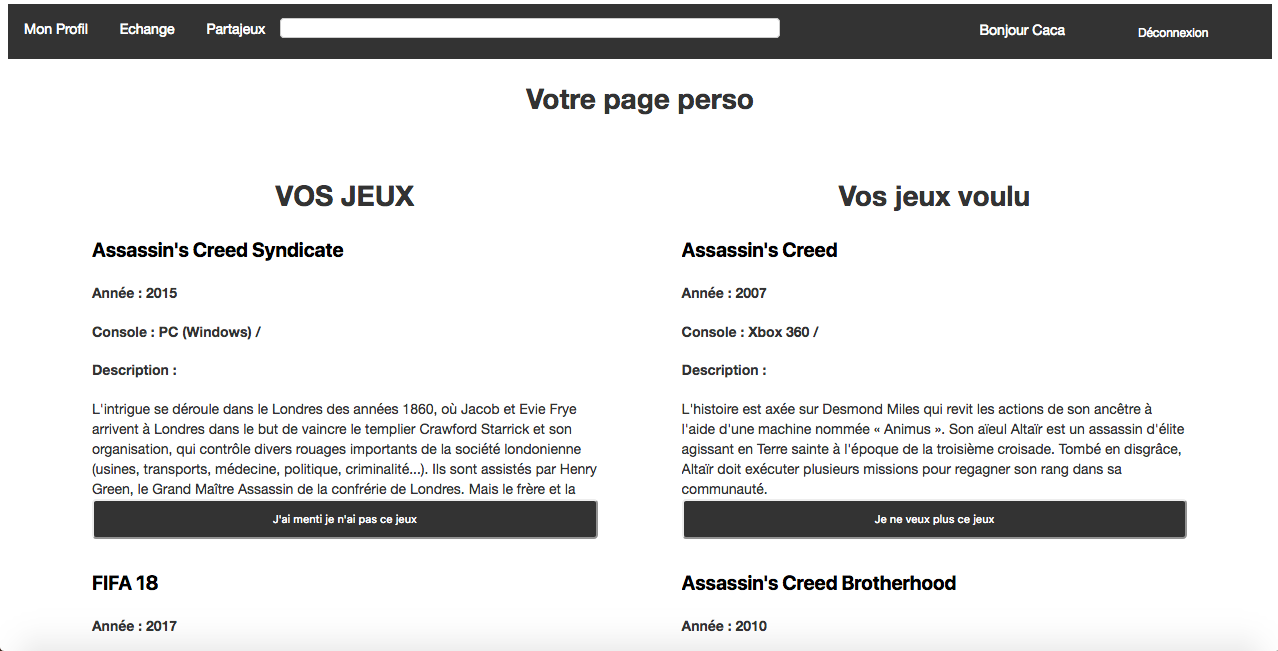
\includegraphics[width=\textwidth]{./doc/03_profile.png}
	\caption{Page de profil}
	\label{profile}
\end{figure}

\newpage
Sur la page personnelle de l'utilisateur il peut voir les jeux qu'il propose pour un échange et à gauche les jeux qu'il aimerait emprunter. L'utilisateur peut également retirer des jeux d'une liste en appuyant sur le bouton approprié.\\

\vspace{1cm}
\begin{figure}[h]
  \centering
    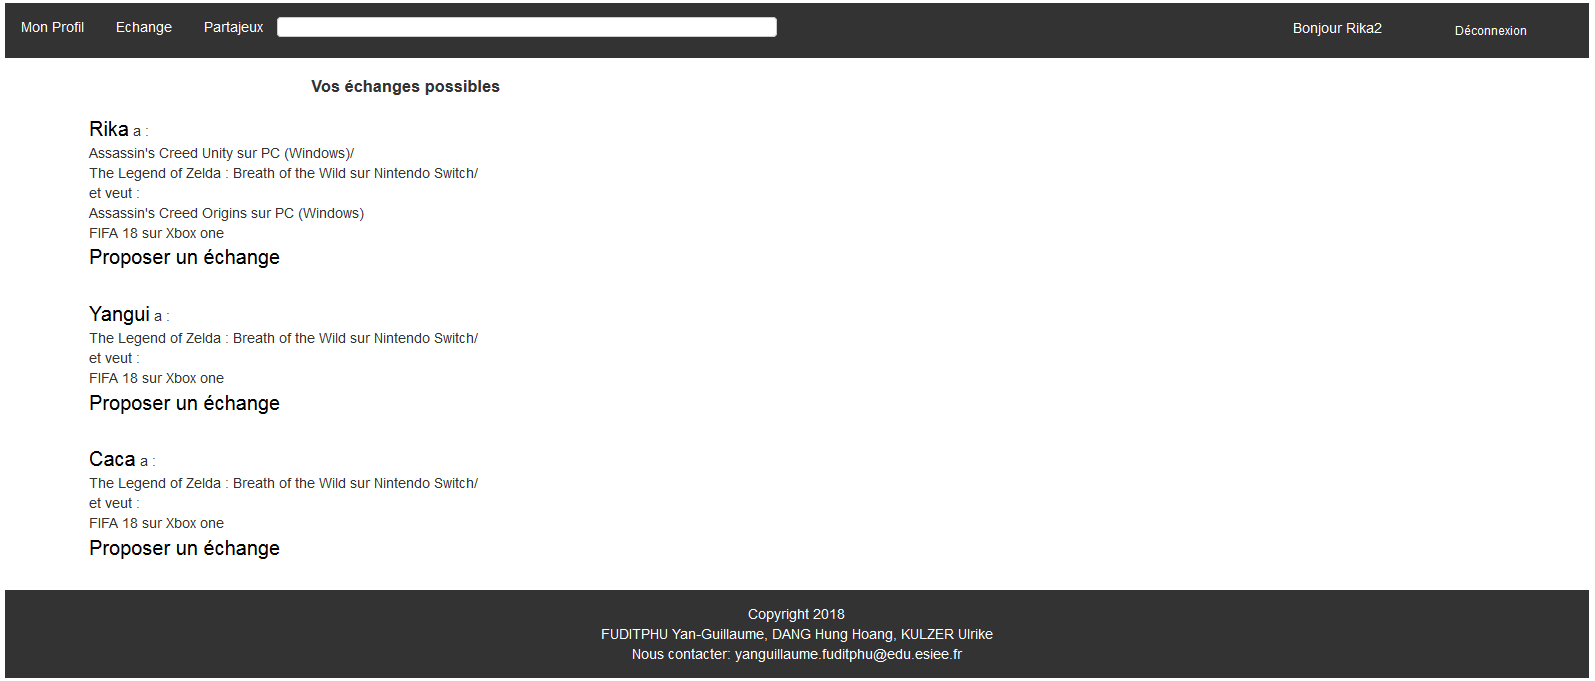
\includegraphics[width=\textwidth]{./doc/04_echanges.png}
	\caption{Échanges possibles}
	\label{exch}
\end{figure}

Si l'utilisateur veut voir ses échanges possibles il clique sur "Échange" et une liste des échanges possibles s'affichera. Chaque proposition suit l'organisation suivante:\\

\begin{quote}
{[utilisateur]} a :\\
{[jeu 1]} sur {[console 1]}\\
{[jeu 2]} sur {[console 2]}\\
...\\
et veut :\\
{[jeu 1]} sur {[console 1]}\\
{[jeu 2]} sur {[console 2]}\\
...\\
Proposer un échange\\
\end{quote}

L'utilisateur peut ensuite cliquer sur le nom de l'utilisateur proposé pour regarder tous les jeux qu'il propose ou lancer l'échange en cliquant sur "Proposer un échange". Par la suite un dialogue va s'afficher dans lequel l'utilisateur peut choisir les jeux proposés pour un échange. Lorsque l'utilisateur a choisi une demande d'échange va être envoyé à l'autre utilisateur qui doit le confirmer.

\newpage
\subsection{Fonctionnalités non réalisées}
\begin{itemize}
\item Proposition d'échange par console :\\
L'application actuellement ne propose aux utilisateurs que les échanges qui sont possibles (basé sur ce qu'ils veulent et possèdent).
\item Confirmation et création d'un échange : L'application n'a pas pu être finalisée faute de temps, en ce moment l'utilisateur ne recevra pas de proposition d'échange.
\item Responsivité du site : Par faute de temps aussi le site n'est pas responsive et n'est donc pas adapté à tous les appareils.
\item Interface BackEnd : Les jeux de la plateforme sont entrés à la main directement dans phpmyadmin. Il faudrait créer une interface afin de permettre aux administrateur de gérer les jeux contenu dans le site.
\end{itemize}

 




%  \begin{minipage}[t]{0.4\linewidth}
 %   \raggedleft
  %  \strut\vspace*{-\baselineskip}\newline\includegraphics[width=0.9\linewidth]{}
    %\caption{décalage de l'alphabet}
   % \label{cesar}
    %\paragraph{}
    %\strut\vspace*{-\baselineskip}\newline\includegraphics[width=0.9\linewidth]{}
    %\caption{tableau de Vigenère}
    %\label{tabVig}
  %\end{minipage}





%{\fbox{\parbox{\textwidth}{\raggedright
%\includegraphics{}}}
%	\captionof{figure}{Écran d'accueil}
%	\label{SP}
%}

%\begin{minipage}[c]{\textwidth}
%\centering
%    \includegraphics[width=\textwidth, trim=1mm 50mm 1mm 1mm, clip]{}
    %TRIM = LINKS UNTEN RECHTS OBEN
%    \captionof{figure}{Structure du programme en modules}
%    \label{img:structure}
%\end{minipage}


%\par
%\vspace{0.5cm}

% "`Standard Definition Television"', HDTV für "`High Definition Television'".


%\begin{itemize}
%\item \blindtext
%\item \blindtext
%\end{itemize}
%\begin{enumerate}
%\item \blindtext
%\item \blindtext
%\end{enumerate}
%\begin{description}
%\item [Ant] \blindtext
%\item [Elephant] \blindtext

%\textbf{greatest} 
%\underline{science} 
%\textbf{\textit{accident}}.


\end{document}




% LABEL UNTER CAPTION

